% Copyright 2006 by Till Tantau
%
% This file may be distributed and/or modified
%
% 1. under the LaTeX Project Public License and/or
% 2. under the GNU Free Documentation License.
%
% See the file doc/generic/pgf/licenses/LICENSE for more details.


\section{Quick Commands}

This section explains the ``quick'' commands of \pgfname. These
commands are executed more quickly than the normal commands of
\pgfname, but offer less functionality. You should use these commands
only if you either have a very large number of commands that need to
be processed or if you expect your commands to be executed very often.


\subsection{Quick Coordinate Commands}

\begin{command}{\pgfqpoint\marg{x}\marg{y}}
  This command does the same as |\pgfpoint|, but \meta{x} and \meta{y}
  must be simple dimensions like |1pt| or |1cm|. Things like |2ex| or
  |2cm+1pt| are not allowed.
\end{command}

\begin{command}{\pgfqpointxy\marg{$s_x$}\marg{$s_y$}}
  This command does the same as |\pgfpointxy|, but \meta{$s_x$} and \meta{$s_y$}
  must be simple numbers without unit, like |1.234| or |5.0|. Mathematical expressions or units are not allowed.
\end{command}

\begin{command}{\pgfqpointxyz\marg{$s_x$}\marg{$s_y$}\marg{$s_z$}}
  As |\pgfqpointxy|, but for three-dimensional coordinates. Any argument needs to be a number without unit.
\end{command}

\begin{command}{\pgfqpointscale\marg{factor}\marg{coordinate}}
	As |\pgfpointscale|, but \marg{factor} must be a simple number without unit, as for the other ``quick'' commands.
\end{command}

\subsection{Quick Path Construction Commands}

The difference between the quick and the normal path commands is that
the quick path commands
\begin{itemize}
\item
  do not keep track of the bounding boxes,
\item
  do not allow you to arc corners,
\item
  do not apply coordinate transformations.
\end{itemize}

However, they do use the soft-path subsystem (see
Section~\ref{section-soft-paths} for details), which allows you to mix
quick and normal path commands arbitrarily.

All quick path construction commands start with |\pgfpathq|.

\begin{command}{\pgfpathqmoveto\marg{x dimension}\marg{y dimension}}
  Either starts a path or starts a new part of a path at the coordinate
  $(\meta{x dimension},\meta{y dimension})$. The coordinate is
  \emph{not} transformed by the current coordinate transformation
  matrix. However, any low-level transformations apply.

\begin{codeexample}[]
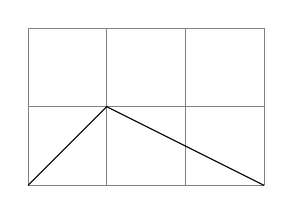
\begin{tikzpicture}
  \draw[help lines] (0,0) grid (3,2);
  \pgftransformxshift{1cm}
  \pgfpathqmoveto{0pt}{0pt} % not transformed
  \pgfpathqlineto{1cm}{1cm} % not transformed
  \pgfpathlineto{\pgfpoint{2cm}{0cm}}
  \pgfusepath{stroke}
\end{tikzpicture}
\end{codeexample}
\end{command}

\begin{command}{\pgfpathqlineto\marg{x dimension}\marg{y dimension}}
  The quick version of the line-to operation.
\end{command}

\begin{command}{\pgfpathqcurveto\marg{$s^1_x$}\marg{$s^1_y$}\marg{$s^2_x$}\marg{$s^2_y$}\marg{$t_x$}\marg{$t_y$}}
  The quick version of the curve-to operation. The first support point
  is $(s^1_x,s^1_y)$, the second support point is  $(s^2_x,s^2_y)$,
  and the target is $(t_x,t_y)$.
 
\begin{codeexample}[]
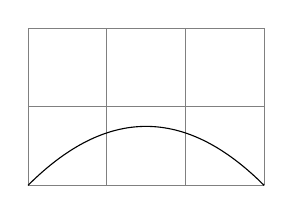
\begin{tikzpicture}
  \draw[help lines] (0,0) grid (3,2);
  \pgfpathqmoveto{0pt}{0pt}
  \pgfpathqcurveto{1cm}{1cm}{2cm}{1cm}{3cm}{0cm}
  \pgfusepath{stroke}
\end{tikzpicture}
\end{codeexample}
\end{command}

\begin{command}{\pgfpathqcircle\marg{radius}}
  Adds a radius around the origin of the given \meta{radius}. This
  command is orders of magnitude faster than
  |\pgfcircle{\pgfpointorigin}{|\meta{radius}|}|. 
 
\begin{codeexample}[]
\begin{tikzpicture}
  \draw[help lines] (0,0) grid (1,1);
  \pgfpathqcircle{10pt}
  \pgfsetfillcolor{examplefill}
  \pgfusepath{stroke,fill}
\end{tikzpicture}
\end{codeexample}
\end{command}



\subsection{Quick Path Usage Commands}

The quick path usage commands perform similar tasks as |\pgfusepath|,
but they
\begin{itemize}
\item
  do not add arrows,
\item
  do not modify the path in any way, in particular,
\item
  ends are not shortened,
\item
  corners are not replaced by arcs.
\end{itemize}

Note that you \emph{have to} use the quick versions in the code of
arrow tip definitions since, inside these definition, you obviously do
not want arrows to be drawn.

\begin{command}{\pgfusepathqstroke}
  Strokes the path without further ado. No arrows are drawn, no
  corners are arced.

\begin{codeexample}[]
\begin{pgfpicture}
  \pgfpathqcircle{5pt}
  \pgfusepathqstroke
\end{pgfpicture}
\end{codeexample}
\end{command}

\begin{command}{\pgfusepathqfill}
  Fills the path without further ado.
\end{command}

\begin{command}{\pgfusepathqfillstroke}
  Fills and then strokes the path without further ado.
\end{command}

\begin{command}{\pgfusepathqclip}
  Clips all subsequent drawings against the current path. The path is
  not processed.
\end{command}


\subsection{Quick Text Box Commands}

\begin{command}{\pgfqbox\marg{box number}}
  This command inserts a \TeX\ box into a |{pgfpicture}| by
  ``escaping'' to \TeX, inserting the box number \meta{box number} at
  the origin, and then returning to the typesetting the picture.
\end{command}

\begin{command}{\pgfqboxsynced\marg{box number}}
  This command works similarly to the |\pgfqbox| command. However,
  before inserting the text in \meta{box number}, the current
  coordinate transformation matrix is applied to the current canvas
  transformation matrix (is it ``synced'' with this matrix, hence the
  name).

  Thus, this command basically has the same effect as if you first
  called |\pgflowlevelsynccm| followed by |\pgfqbox|. However, this
  command will use |\hskip| and |\raise| commands for the
  ``translational part'' of the coordinate transformation matrix,
  instead of adding the translational part to the current
  canvas transformation matrix directly. Both methods have the same
  effect (box \meta{box number} is translated to where it should be), but
  the method used by |\pgfqboxsynced| ensures that hyperlinks are
  placed correctly. Note that scaling and rotation will not (cannot,
  even) apply to hyperlinks.
\end{command}

%%% Local Variables: 
%%% mode: latex
%%% TeX-master: "pgfmanual"
%%% End: 
